\cleardoublepage

\chapter{Arquitecturas asimétricas y heterogéneas}
\label{ch:chapter2}

\section{Descripción general del paradigma big.LITTLE}

\subsection{Soporte en el kernel para arquitecturas big.LITTLE}
\label{sec:models}

Las arquitecturas big.LITTLE modernas ofrecen un conjunto de distintos modelos de ejecución
soportados por el sistema operativo (algunos de ellos exigen soporte también a nivel de
hardware):

\begin{description}

	\item[Cluster Switching Mode (CSM)]

El procesador se divide de forma lógica en dos clusters, uno conteniendo los núcleos
rápidos, y otro conteniendo los núcleos lentos, pero sólo uno de ellos es utilizable
simultáneamente en tiempo de ejecución. El sistema operativo activa/desactiva los 
clusters de forma transparente, en función de la carga de trabajo, para equilibrar
el rendimiento y la eficiencia energética.

	\item[CPU migration (CPUM)]

Los núcleos físicos se agrupan en pares, cada uno formado por un núcleo rápido y otro
lento, construyendo {\em Núcleos Virtuales (VC)}, a los que el sistema operativo mapea
hebras. En un instante determinado, sólo un núcleo físico está activo por VC, dependiendo
de los requisitos exigidos por la carga computacional activa. En aquellas implementaciones
big.LITTLE en las que el número de núcleos lentos y rápidos no es el mismo, cada VC puede
estar formado por diferente número de núcleos de cada tipo. La solución implementada
por Linaro en el kernel de Linux se conoce como {\em In-Kernel Switcher (IKS)}~\cite{}.

	\item[Global Task Scheduling (GTS)]

Se trata del modelo más flexible. Todos los núcleos (lentos y rápidos) están disponibles
para la planificación de hebras, y el sistema operativo las mapea en función de la naturaleza
de la carga computacional asociada a cada uno de ellos y la disponibilidad de núcleos. 

\end{description}

\begin{figure}%[tbh!]
 \centering
  \begin{subfigure}{.75\textwidth}
   \centering
   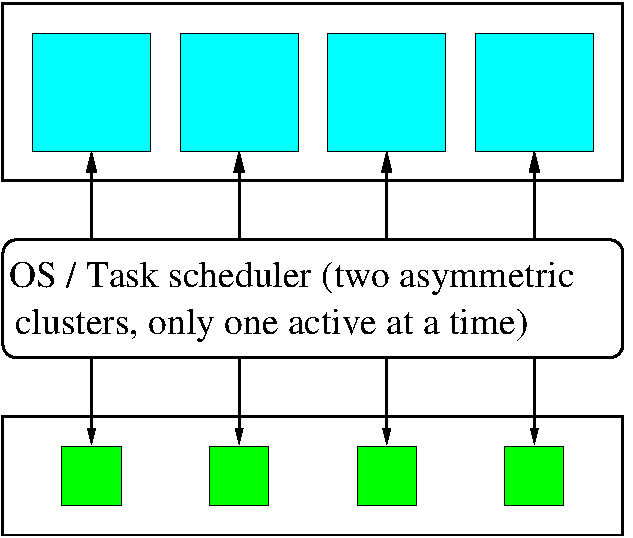
\includegraphics[width=0.4\textwidth]{Figures/Models/clustered.pdf}
   \caption{CSM}
  \end{subfigure}

	\medskip

  \begin{subfigure}{.75\textwidth}
   \centering
   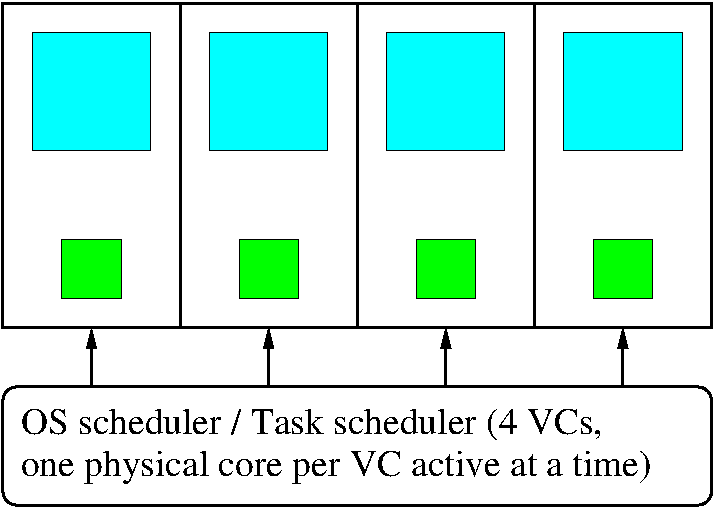
\includegraphics[width=0.45\textwidth]{Figures/Models/iks.pdf}
   \caption{CPUM}
  \end{subfigure}

	\medskip

  \begin{subfigure}{.75\textwidth}
   \centering
   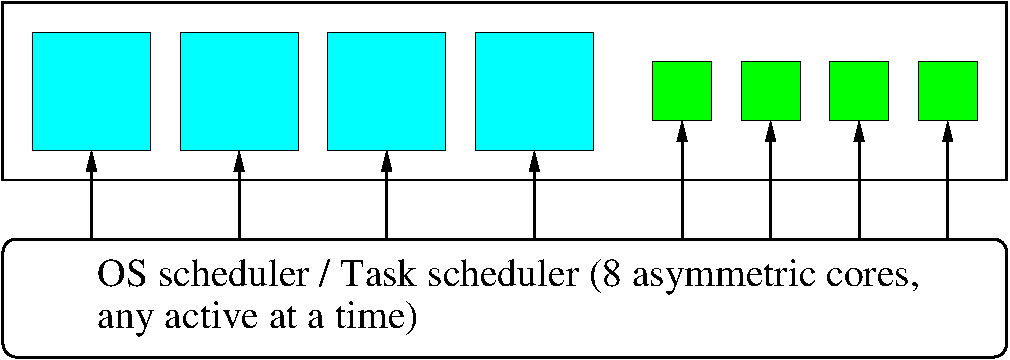
\includegraphics[width=0.6\textwidth]{Figures/Models/gts.pdf}
   \caption{GTS}
  \end{subfigure}
   \caption{Modos de operación de las arquitecturas big.LITTLE actuales.}
   \label{fig:modes}
\end{figure}

\comentario{Falta traducir figura}


La Figura~\ref{fig:modes} ofrece una visión esquemática de estos tres modelos de ejecución
sobre arquitecturas big.LITTLE modernas. GTS es la solución más flexible, ya que permite al planificador
del sistema operativo asignar hebras a cualquiera de los núcleos disponibles, es decir, todos
los núcleos disponibles se ofrecen al sistema operativo como candidatos a ejecutar el código
de cualquier hebra, independientemente de su naturaleza o características. Esta característica
permite migrar de forma muy sencilla aplicaciones multihebra ya existentes, incluyendo planificadores
de tareas en tiempo de ejecución, y explotar todos los recursos computacionales en este tipo de 
procesadores asimétricos, utilizando cualquier mecanismo estándar de creación y gestión de hebras
(por ejemplo, pthreads u OpenMP). Sin embargo, conseguir prestaciones óptimas no resulta tan
sencillo, especialmente en aplicaciones multihebra en las que el desequilibrio de carga introducido
por la asimetría de la arquitectura puede penalizar el rendimiento obtenido. Solucionar este problema
es uno de los objetivos de este trabajo.

De forma alternativa, CPUM propone una visión pseudosimétrica del procesador big.LITTLE; por ejemplo,
en el caso del SoC Exynos 5422, los 8 núcleos asimétricos son vistos de forma lógica como 4 grupos
de pares de procesadores, convirtiendo así la arquitectura en un sistema simétrico formado por
4 núcleos virtuales (VC), que son expuestos de esta manera al sistema operativo.

En la práctica, los planificadores de tareas en tiempo de ejecución pueden aproximar a nivel software
cualquiera de estos tres paradigmas. Un modelo trivial puede seguir las directivas de GTS para asignar
cualquier tarea lista para su ejecución a cualquiera de los núcleos disponibles en el sistema. Con esta
solución, el desequilibrio de carga podría resolverse desarrollando políticas de planificación a nivel
de tarea específicas (conscientes de la asimetría), para asignar tareas al recurso más apropiado en 
función de sus características. 

Sin embargo, este trabajo propone un enfoque alternativo, en el que el SoC asimétrico es visto de forma
lógica como un conjunto {\em simétrico} de núcleos virtuales, cada uno de ellos compuesto internamente
por distintos tipos de núcleo, pero considerado, de cara al planificador, como un sistema simétrico. Esto
facilita el desarrollo de políticas de planificación, como se verá más adelante, y permite incluso
reutilizar planificadores ya existentes sobre este tipo de arquitecturas.

\section{Descripción del entorno experimental}

\subsection{ODROID}

\subsection{Juno}

\subsection{Software utilizado}

\subsection{Entorno de medición de consumo}


%-- Configuraciones para emacs --
%%% Local Variables:
%%% mode: latex
%%% TeX-master: "./principal.tex"
%%% End:
